Um ein besseres Verständnis zu ermöglichen, wird zunächst auf die generelle Funktionsweise von Maven näher eingegangen.

\subsubsection{Workflow Maven}
Innerhalb Maven sind Strukuren oder Abläufe, die zur Kompilierung, Testen, Paketierung und Veröffentlichung von Projekten benötigt werden, bereits vorgegeben und müssen nicht mehr definiert werden. \cite[S. 27]{spiller_maven_2011} Dies erleichtert insbesondere die Verwaltung von Projektabhängigkeiten, da Bibliotheken einfach ausgetauscht werden können und die entsprechenden Abhängigkeiten sowie die transitiven Abhängigkeiten aufgelöst und entfernt werden. In Abbildung 23 wird die generelle Funktionsweise von Maven dargestellt und auf besondere Eigenschaften näher eingegangen. 

\begin{figure}[h]
    \centering
    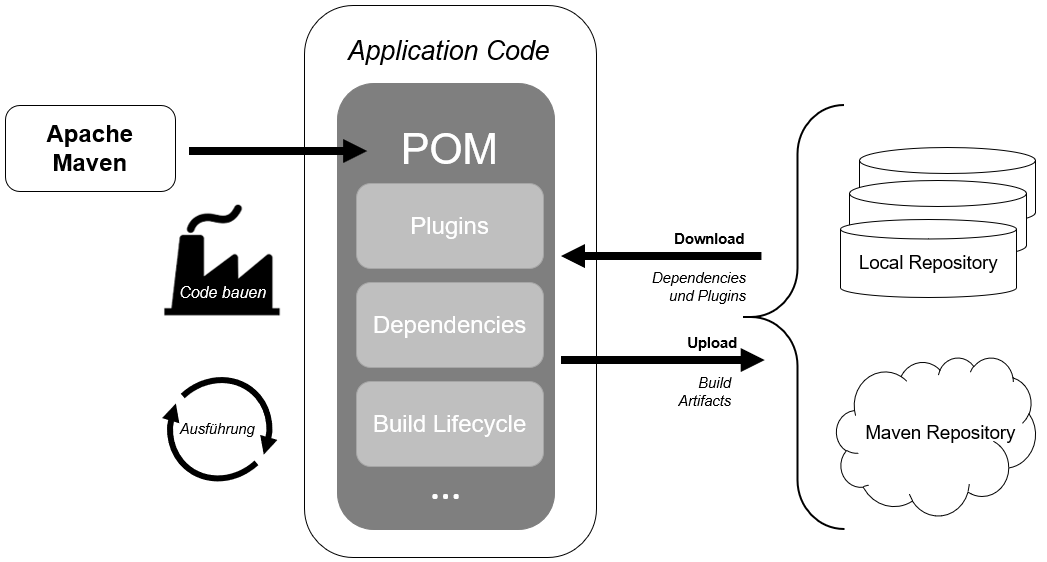
\includegraphics[scale=0.5]{Bilder/Workflow_Maven.png}
    \caption{Funktionsweise von Maven, angelehnt an \cite{guntur_understanding_2020}}
\end{figure}

\paragraph{4.2.1.1. POM} $~$
 
Die Funktionsweise und die Verwaltung des Projektes baut grundsätzlich auf dem 'Project Object Model' (kurz: POM) auf und bildet daher den Kern eines jeden Maven-Projektes ab. Ferner bietet Maven die Möglichkeit Projektabhängigkeiten, Projektumgebungen und Projektbeziehungen in einer seperaten, externen pom.xml-Datei, die während des Build-Prozesses verwendet werden sollen zu deklarieren. \cite[S. 3]{varanasi_introducing_2019}\cite{the_apache_software_foundation_maven_2002} Zudem erzeugt Maven Artefakte, die einzeln ausgeliefert und in die Repositorys übertragen werden. \cite[S. 29]{spiller_maven_2011}

\paragraph{4.2.1.2.Repository} $~$

Ferner verwendet Maven Repositorys. Innerhalb des Local Repositorys werden alle Abhängigkeiten abgelegt, die für die Erstellung des Builds benötigt werden. Zunächst überprüft Maven, ob sich benötigten Abhängigkeiten bereits innerhalb des Local Repositorys befinden. \cite[S. 45 - 47]{loukides_maven_2008} Ist dies der Fall, wird die Datei, ohne die Erstellung einer Kopie im lokalen Verzeichnis, innerhalb des Local Repositorys verwendet, ansonsten versucht Maven die Datei auf das Local Repository herunterzuladen und zu kopieren, um diese aussschließlich lokal verwendet zu können. \cite[S. 115]{spiller_maven_2011}   

\paragraph{4.2.1.3. Build-Lifecycle} $~$

Prinzipiell sind Lifecycles abstrahierte Arbeitsschritte innerhalb festen Phasen, die in einer bestimmten Reihenfolge durchlaufen und für den Build-Prozess essentiell sind. \cite[S. 57]{varanasi_introducing_2019} 
Maven definiert dabei drei Lifecycles\cite[S. 72 - 76]{spiller_maven_2011}: 

\begin{itemize}
    \item \textit{clean}: Löschung, was keine Notwendigkeit mehr hat 

    \item \textit{site}: Erzeugen von Projektdokumentationen
    
    \item \textit{build/default}: Standardisierter Ablauf zum Erzeugen einer Anwendung 

\end{itemize}

Sobald Maven die einzelnen Phasen eines Lifecycles durchläuft, wie in der Abbildung 24 zu erkennen ist, werden die Ziele jedes Plugins ausgeführt, die mit jeder einzelnen Phase verbunden sind. \cite[S. 39]{loukides_maven_2008} 

\begin{figure}[h]
    \centering
    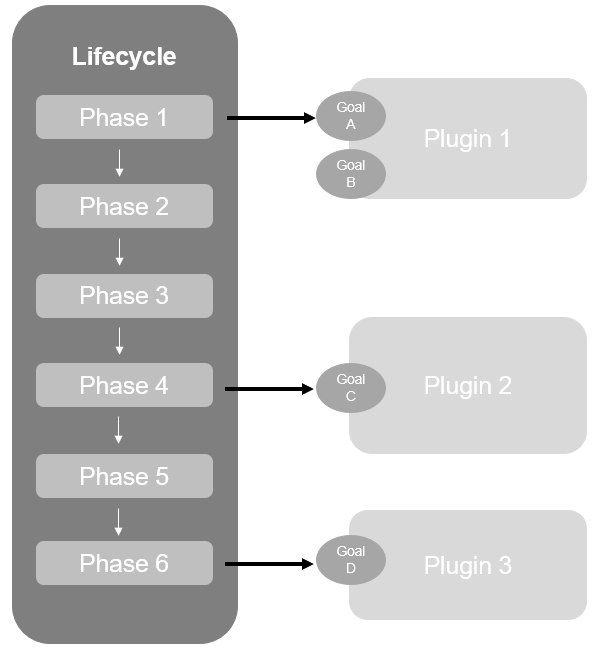
\includegraphics[scale=0.4]{Bilder/lifecycle_maven.png}
    \caption{Zusammenspiel Plugin-Goals und Lifecycle, \cite[S. 59]{varanasi_introducing_2019}}
\end{figure}

\paragraph{4.2.1.4. Plugins in Maven} $~$

Maven ist ein Framework zum Ausführen von Plugins, indem benötigte Funktionen als Plugins anhand des Goals in den Softwareentwicklungsprozess ausgeführt werden. Infolgedessen kann jede Funktionalität durch ein Plugin ersetzt werden, womit Plugins eine zentrale Rolle innerhalb des Softwareentwicklungsprozesses zufällt. Mittels der Auslagerung unterschiedlicher Aufgaben, ist sowohl der Einsatz als auch die Wartung einfacher wie bei großen Abhängigkeiten, da die Aktualisierung durch Maven durchgeführt werden.  

\subsubsection{Entwurf des PoC basierend auf dem Ayoy - Maven Licence Vertify Plugin}

Kernelement des Ayoy-Plugins ist die Prüfung und der darauf aufbauende Vergleich von Lizenzmodellen und deren Abhängigkeiten innerhalb eines Projektes.

\begin{figure}[h]
    \centering
    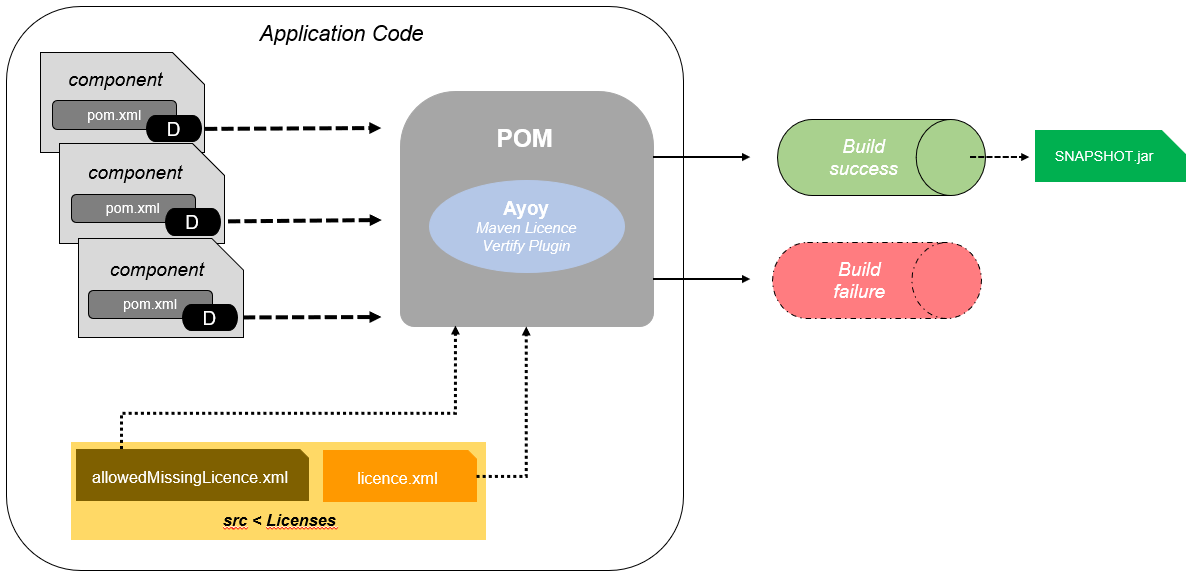
\includegraphics[scale=0.4]{Bilder/Ayoy-Plugin.png}
    \caption{Funktionsweise des Ayoy-Plugin}
\end{figure}

Anhand der Abbildung 25 wird zunächst die generelle Funktionsweise schemenhaft dargestellt, um ein besseres Verständnis des Workflows dieses Plugins zu erhalten. Alle Komponeten des ausführbaren Programms beinhalten zunächst jeweils eine pom.xml-Datei und die darin enthaltenen Bibliotheken als zu prüfende Abhängigkeiten. Eine pom.xml enthält neben der groupId, artifactId und version zur Identifikation, die Lizenz des Projektes, verschiedene Abhängigkeiten und die entsprechenden Plugins, die zur Ausführung benötigt werden. Die für den Vergleich essentielle licence.xml, befindet sich src-Verzeichnis eines jeden Programmes und muss dementsprechend, in jedem Programm hinterlegt werden. Die darin enthaltenen Lizenzmodelle werden jeweils mit Namen und der dazu gehörigen URL versehen. Die Angabe der URL muss zwingend eingehalten werden, da der Vergleich auf diesem Wert basiert, während der Name aussschließlich für die Ausgabe verwendet wird. Ist keine URL einer Lizenz vorhanden, wird ein Fehler angezeigt. Die licence-Datei wird als ein xml-Format gespeichert und enthält alle erlaubten ('valid') und nicht genehmigten ('forbidden') Lizenzmodelle, wie in der Abbildung 26 dargestellt. 

\begin{figure}[h]
    \centering
    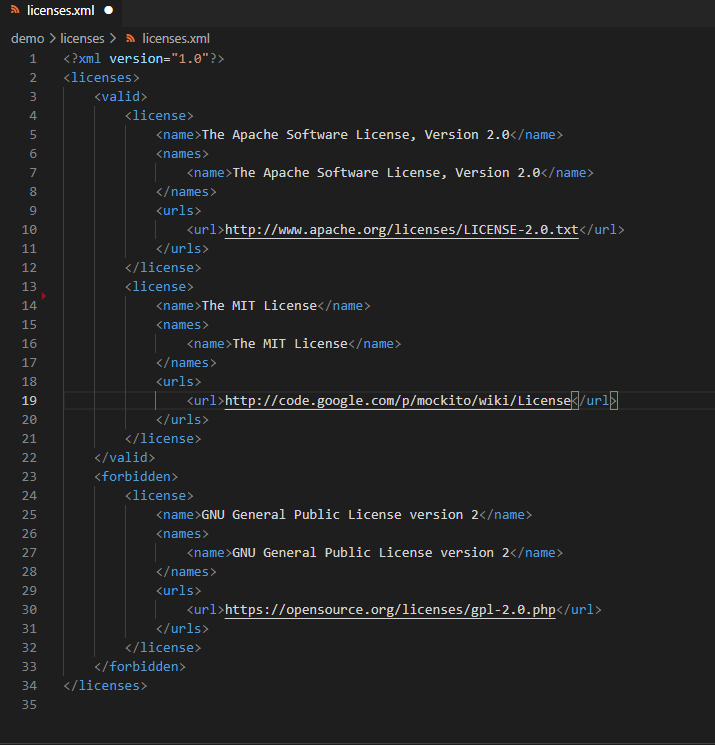
\includegraphics[scale=0.45]{Bilder/licencesxml.png}
    \caption{Genehmigte und nicht genehmigte Lizenzmodelle innerhalb der licence.xml}
\end{figure}

Nachdem der Build-Prozess angestoßen wird, vergleicht das Plugin alle Lizenzen der unterschiedlichen pom.xml-Dateien und deren Abhängigkeiten des aktuellen Projekts mit der entsprechenden licence.xml. Wenn die Anforderungen erfüllt sind, wird der Build-Prozess erfolgreich ausgeführt, ansonsten wird dieser abgebrochen, wie anhand der Abbildung 25 zu sehen ist.\\ Ferner kann der Build-Prozess unterschiedlich gestartet werden. Sollte das Plugin, gemäß der Anforderungsdefinition, automatisiert und daher regelmäßig durchgeführt werden, muss der entsprechende Aufruf innerhalb der pom.xml konfiguriert werden, wie Abbildung 27 zeigt. 

\begin{figure}[h]
    \centering
    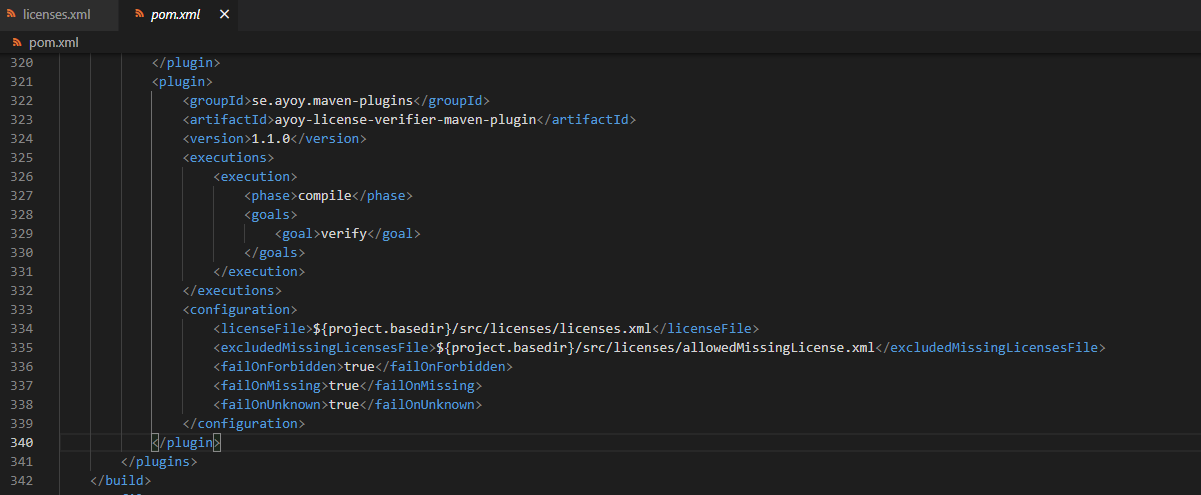
\includegraphics[scale=0.45]{Bilder/PluginConfigurationzumAufruf.png}
    \caption{Eingebunder Aufruf innerhalb der pom.xml}
\end{figure}

Bei unregelmäßiger Verwendung kann der Aufruf, anhand Abbildung 28 ersichtlich, über die Kommandozeile mittels folgenden Befehl eingegeben werden:  

\begin{figure}[h]
    \centering
    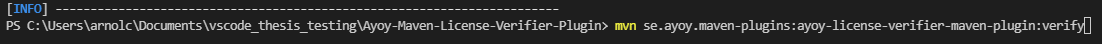
\includegraphics[scale=0.5]{Bilder/mvn-Aufruf.png}
    \caption{Aufruf der pom.xml innerhalb der Kommandozeile}
\end{figure}

Der Aufruf spiegelt den Pfad des Goals des Plugins innerhalb des Repositorys dar: 

\begin{itemize}
    \item \textbf{mvn}: Syntax zum Ausführen des Maven-Befehls
    \item \textbf{se.ayoy.maven-plugins}: Aufruf der Bibliothek innerhalb des Repositorys
    \item \textbf{ayoy-license-verifier-maven-plugin}: Aufruf des Plugins auf dem Repositorys
    \item \textbf{verify}: Goal des Plugins
\end{itemize}

Die Prüfung der Abhängigkeiten ist neben der Prüfung der direkten Lizenzen von Komponenten essentiell, da Bibliotheken ebenfalls Lizenzmodelle besitzen, die ein starkes Copyleft aufweisen können und aufgrund dessen von dem Plugin erkannt werden. Ferner prüft das Plugin zudem eingebundene Abhängigkeiten, die weitere Abhängigkeiten aufweisen und diese widerrum ein risikoreiches Copyleft beinhalten können. In diesem Rahmen besteht die Möglichkeit, dass sich die Lizenzen der Abhängigkeiten aufgrund einer Versionsänderung auf ein Lizenmodel mit beschränkter oder starker Copyleft umgestellen. Sowohl Versionsumstellungen als auch transitive Abhängigkeiten sind oftmals für den Entwickler nicht sofort erkennbar und bieten ein hohes Potential 'gefährliche' Lizenzmodelle zu übersehen. Während transitive Abhängigkeiten zwingend betrachtet werden müssen, sollten Abhängigkeiten die aussschließlich zum Testen verwendet werden, nicht innerhalb des Plugins einbezogen werden, sowie innerhalb des Kapitels 3.2.1. in Szenario eins beschrieben wurde. Da diese Abhängigkeiten aussschließlich für Testzwecke verwendet und folglich nicht ausgeliefert werden, ist eine Beachtung der Lizenzmodelle nicht zwingend notwendig. 

\begin{figure}[h]
    \centering
    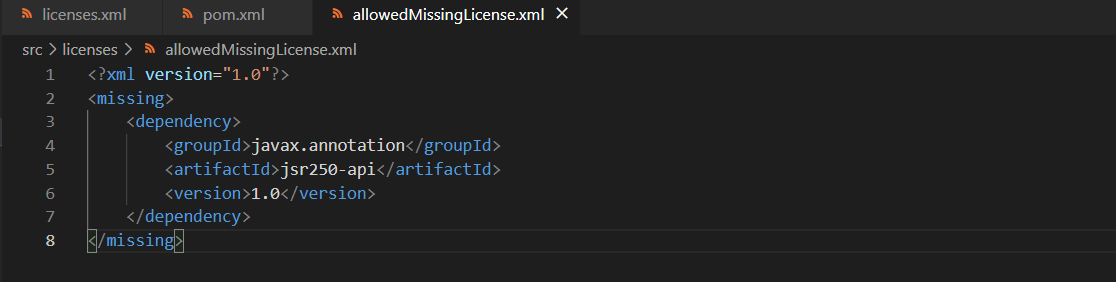
\includegraphics[scale=0.5]{Bilder/allowedmiisingLicence.png}
    \caption{Zu Testzwecken eingebettete Abhängigkeit innerhalb der allowedMissingLicence.xml}
\end{figure}

Zu diesem Zweck müssen die entsprechenden Lizenzen zunächst innerhalb der allowedMissingLicence.xml eingebettet werden, wie in Abbildung 29 dargestellt. Die Lizenzmodelle der darin eingegebenen Abhängigkeiten werden vom Plugin ignoriert, ohne das Build-Prozess fehlschlägt, falls eine risikoreiche Lizenzen gefunden wird. Als Ergebnis des Build-Prozesses wird die SNAPSHOT.jar als eine ausführbare Datei erstellt. 








% Die POM muss drei wesentliche Tags enthalten \cite[S. 77 - 78]{spiller_maven_2011}: 

% \begin{itemize}
%     \item \textit{groupId}: Enthält eine eindeutige, identifizierbare Bezeichnung für ein Projekt
%     \item \textit{artifactId}: Enthält eine eindeutige, identifizierbare Bezeichnung für ein Artefakt bzw. Projekt pro groupId
%     \item \textit{version}: Enthält die aktuelle Version des Artefakts
% \end{itemize}








